\begin{figure}
\definecolor{hllorange}{rgb}{.8,0,0}
\centering
	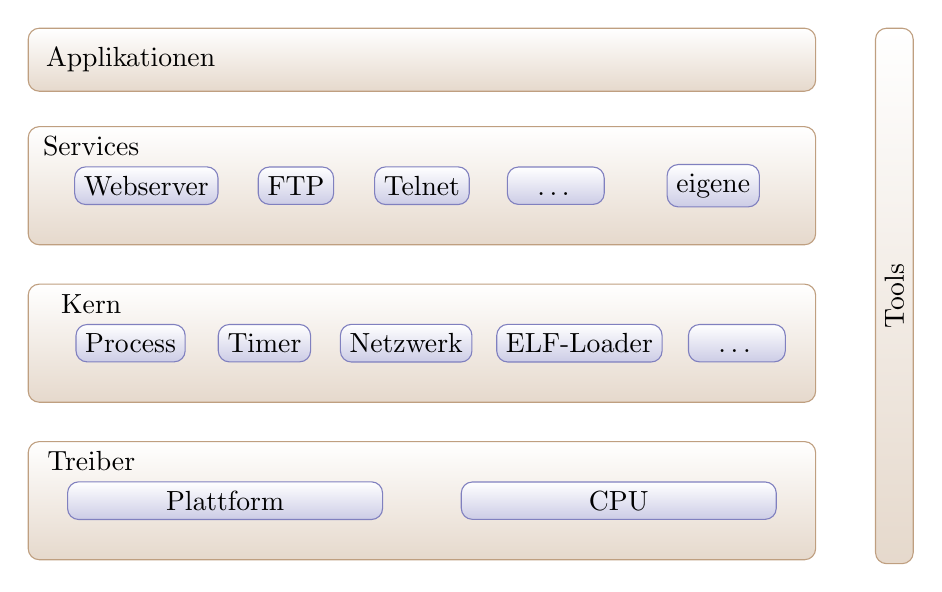
\begin{tikzpicture}
		\tikzstyle{subele}=[draw,
			rounded corners,
			top color=white,
			bottom color=blue!50!black!20,
			draw=blue!50!black!50,
			];
		\tikzstyle{ele}=[draw,
			rounded corners,
			top color=white,
			bottom color=orange!50!black!20,
			draw=orange!50!black!50,
			];

		\node [ele] at (0,5.6) [minimum width=10cm,minimum height=.8cm] {};
		\node at (-3.7,5.6) {Applikationen};

		\node [ele] at (0,4) [minimum width=10cm,minimum height=1.5cm] {};
		\node at (-4.2,4.5) {Services};
		\node [subele] at (-3.5,4) {Webserver};
		\node [subele] at (-1.6,4) {FTP};
		\node [subele] at (0,4) {Telnet};
		\node [subele] at (1.7,4) {\phantom{A}\dots\phantom{A}};
		\node [subele] at (3.7,4) {eigene};

		\node [ele] at (0,2) [minimum width=10cm,minimum height=1.5cm] {};
		\node at (-4.2,2.5) {Kern};
		\node [subele] at (-3.7,2) {Process};
		\node [subele] at (-2.0,2) {Timer};
		\node [subele] at (-.2,2) {Netzwerk};
		\node [subele] at (2,2) {ELF-Loader};
		\node [subele] at (4,2) {\phantom{A}\dots\phantom{A}};

		\node [ele] at (0,0) [minimum width=10cm,minimum height=1.5cm] {};
		\node at (-4.2,.5) {Treiber};
		\node [subele] at (-2.5,0) [minimum width=4cm] {Plattform};
		\node [subele] at (2.5,0) [minimum width=4cm] {CPU};

		\node [ele] at (6,2.6) [minimum width=6.8cm,rotate=90] {Tools};
	\end{tikzpicture}
	\captionbelow[Contiki-Schichten]{Contiki-Schichten nach \autocite{dreier10contikiblackfin}}
\label{fig:contiki_schichten}
\end{figure}
